\documentclass[12pt]{article}

% Full article preamble (duplicated, no common file)
\usepackage{fontspec}
\usepackage[a4paper,margin=2.5cm,includefoot]{geometry}
\usepackage{polyglossia}
\usepackage{amsmath}
\usepackage{amssymb}
\usepackage{xcolor}
\usepackage{fancyhdr}
\usepackage{graphicx}
\usepackage{listings}
\usepackage[most]{tcolorbox}
\usepackage{pifont}
\usepackage{enumitem}
\usepackage{titlesec}
\usepackage[bottom]{footmisc}
\usepackage{titling}
\usepackage{minted}
\usepackage{etoolbox}
\usepackage{array}
\usepackage{extsizes}

\newfontfamily\emoji{Segoe UI Emoji}

\pagestyle{fancy}

\setmainlanguage[numerals=western]{arabic}
\setotherlanguage{english}
\newfontfamily\arabicfont[Script=Arabic]{Amiri}
\newfontfamily\arabicfonttt[Script=Arabic]{Courier New}

\lstset{
  language=[Sharp]C,
  numbers=left,
  stepnumber=1,
  numbersep=8pt,
  frame=single,
  basicstyle=\ttfamily\small,
  keywordstyle=\color{blue},
  stringstyle=\color{red},
  commentstyle=\color{green!50!black}
}

\newif\ifdetailed
\ifdefined\setdetailed
  \setdetailed
\fi

\newif\ifwithsols
\ifdefined\setwithsols
  \setwithsols
\fi

% unified tcolorboxes for articles
\tcbset{colback=white, colframe=black, fonttitle=\bfseries, boxrule=0.8pt}
\newtcolorbox{boxDef}[1][]{colback=blue!5!white,colframe=blue!75!black,
  title={{\emoji📘} تعريف\ifx\\#1\\\else ~#1\fi :}}
\newtcolorbox{boxExercise}[1][]{colback=cyan!5!white,colframe=cyan!70!black,
  title={{\emoji🧩} تمرين\ifx\\#1\\\else ~#1\fi :}}
\newtcolorbox{boxExample}[1][]{colback=yellow!5!white,colframe=orange!90!black,
  title={{\emoji📝} مثال\ifx\\#1\\\else ~#1\fi :}}
\newtcolorbox{boxNote}[1][]{colback=gray!10!white,colframe=black,
  title={{\emoji✨} ملاحظة\ifx\\#1\\\else ~#1\fi :}}
\newtcolorbox{boxAttention}[1][]{colback=magenta!10!white,colframe=magenta!80!black,
  title={{\emoji🔔} تنبيه\ifx\\#1\\\else ~#1\fi :}}
\newtcolorbox{boxWarning}[1][]{colback=red!5!white,colframe=red!75!black,
  title={{\emoji⚡} ملاحظة هامة\ifx\\#1\\\else ~#1\fi :}}
\newtcolorbox{boxSolution}[1][]{colback=green!5!white,colframe=green!60!black,
  title={{\emoji✅} حل\ifx\\#1\\\else ~#1\fi :}}
\newtcolorbox{boxSymbol}[1][]{colback=purple!5!white,colframe=purple!70!black,
  title={{\emoji🔣} رمز\ifx\\#1\\\else ~#1\fi :}}

\tcbset{simplecode/.style={ colback=gray!5, colframe=black!50, boxrule=0.4pt, arc=2pt, left=4pt,right=4pt,top=4pt,bottom=4pt}}
\newenvironment{boxCode}{\begin{tcolorbox}[simplecode]}{\end{tcolorbox}}

\newcolumntype{C}[1]{>{\centering\arraybackslash}p{#1}}

% redefine spaces after titles
\makeatletter
\renewcommand{\@maketitle}{%
  \begin{center}
    {\huge \bfseries \@title \par}%
    \vskip 0.2em % space between title and author
    {\large \@author \par}%
    % \vskip 0.2em % space between author and date
    % {\normalsize \@date \par}%
  \end{center}
}
\makeatother

\fancyhf{} % clear default
\fancypagestyle{plain}{
  \fancyhf{}
  \fancyhead[L]{مدرسة التسامح الشاملة}
  % \fancyhead[L]{
\includegraphics[height=1cm]{../../../images/logoTasamoh.png}}
  \fancyhead[R]{الأستاذ محمود اغبارية}
  \fancyfoot[C]{\thepage}
}

\fancyhead[L]{مدرسة التسامح الشاملة}
\fancyhead[R]{الأستاذ محمود اغبارية}
\fancyfoot[C]{\thepage}
% \date{\today}

\setcounter{tocdepth}{3} % only section subsection and subsubsection in TOC


% ----------------------


% \begin{document}

% \maketitle

% % \clearpage  % start TOC on a new page
% % \renewcommand{\contentsname}{جدول المحتويات}
% % \tableofcontents
% % \clearpage

% \part*{part 1} % the * prevents numbering
% \section*{مقدمة}
% \subsection*{مثال رياضي}
% \subsubsection*{مثال فرعي}
% \paragraph*{ paragraph 1}
% \subparagraph*{sub paragraph 1}

% \ifdetailed
% \begin{english}
% \begin{minted}{csharp}
% // C# Example
% \end{minted}
% \end{english}
% \fi

% OLD WAY
% \ifdetailed
% \begin{english}
% \begin{lstlisting}
% // C# Example
% \end{lstlisting}
% \end{english}
% \fi

% % 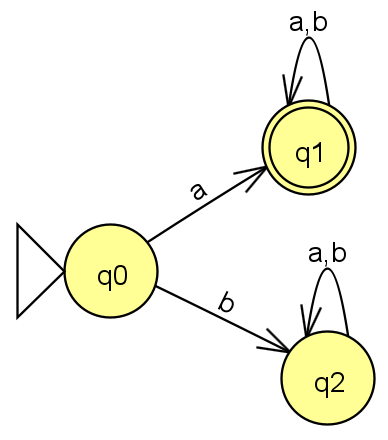
\includegraphics[width=0.2\textwidth]{../../../images/DFAs/ex1_q1.png}



% \vspace{3cm}
% \begin{flushleft}
% أرجو لكم وقتًا ممتعًا.

% الأستاذ محمود اغبارية.
% \end{flushleft}


% \end{document}


\title{قائمة مواد أساسيات علوم الحاسوب بلغة C\# حسب خطة وزارة المعارف}

\begin{document}

\maketitle
\thispagestyle{fancy}


\renewcommand{\contentsname}{جدول المحتويات}
\tableofcontents
\clearpage


\section{المقدمة ومصطلحات أساسية}

\subsection{مقدمة عن الخوارزميات والبرمجة}

انظر عرض "مقدمة" الذي أعددته.

بعده نبدأ بالبرمجة.

\begin{itemize}
\item البدء خطوة بخطوة إلى أن ينشئ الطالب مشروعًا جديدًا في Visual Studio
\item التعريف بمبنى المشروع العام
\item التعريف بمبنى الملف $\mathtt{Program.cs}$ العام
\end{itemize}

\subsection{كتابة إلى الشاشة، وقراءة من المستخدم}

\begin{itemize}
    \item نشرح بأقل الممكن طريقة طباعة متغير على الشاشة أو أي نص
    \item نشرح بأقل الممكن طريقة استقبال عدد من المستخدم
\end{itemize}

\clearpage
\section{المتغيرات}

\begin{enumerate}
    \item  المتغيرات: تعريفها وإعطاؤها قيمة (الاسم والنوع لا يتغيران، القيمة تتغير)
    \item  الأنواع الأساسية للمتغيرات،
    \item  \textit{قوانين أسماء المتغيرات المسموحة}
    \item  \textbf{أهمية اختيار اسم معبّر للمتغير}
    \item  خاصة: $\mathtt{int}$ و $\mathtt{double}$ ومجالات قيم كل نوع (القيم بالبرمجة محدودة وليس كما في العالم غير محدودة)
    \item  العمليات الحسابية على المتغيرات:
    \begin{itemize}
        \item جمع
        \item طرح
        \item ضرب
        \item قسمة
        \item باقي
        \item ترتيب العمليات الحسابية (مع أقواس وبدون)
    \end{itemize}
    \item  تحويل بين الأنواع  $\mathtt{int}$ و $\mathtt{double}$:
    \item تحويل صريح
    \item تحويل ضمني (عند قسمة $\mathtt{int}$ على $\mathtt{double}$ مثلا)
    \item  تعريف المتغير وإعطاؤه قيمة في نفس السطر أو في سطرين مختلفين.
    \item  إعطاء قيمة للمتغير هو نسخ وليس نقل للقيمة
\end{enumerate}

\clearpage
\section{مقدمة قصيرة عن الفئات}

\subsection{الفئات}
\begin{itemize}
    \item تعريف المصطلحات: فئة، كائن، خاصية، عملية
    \item قراءة ملف فئة وفهمه
    \item إنشاء كائن من فئة معينة
    \item استدعاء عمليات فئة معينة
\end{itemize}


\subsection{استدعاء عمليات}

استدعاء عمليات $\mathtt{static}$ من فئة خارجية: $\mathtt{ClassName.MethodName()}$ بأقل تفصيل ممكن (التعامل مع $\mathtt{Math}$ كمجموعة عمليات كتبها شخص آخر ونحن نستدعيها.)

\subsection{عمليات الفئة $\mathtt{Math}$}
\begin{itemize}
    \item $\mathtt{Math.Abs}$
    \item $\mathtt{Math.Max}$
    \item $\mathtt{Math.Min}$
    \item $\mathtt{Math.Pow}$
    \item $\mathtt{Math.Round}$
    \item $\mathtt{Math.Sqrt}$
\end{itemize}

\subsection{الفئة $\mathtt{Random}$ واستخداماتها}

//TODO

\subsection{قراءة ملف فئة وفهمه}
\begin{itemize}
    \item قراء ملف فئة وفهمه
    \item قراءة برنامج يستخدم هذه الفئة وفهمه
    \item تغيير هذا البرنامج للحصول على النتيجة المطلوبة
\end{itemize}

\subsection{التعامل مع متغير النص $\mathtt{String}$}

\begin{itemize}
    \item ربط نصين ببعضهما
    \item تنسيق النص مع متغيرات $\mathtt{\$}$
    \item $\mathtt{int.Parse(Console.ReadLine());}$
    \item $\mathtt{double.Parse(Console.ReadLine());}$
    \item \textbf{موضوع $\mathtt{String}$ ليس مطلوبًا لأول وحدتين، المطلوب فقط التعامل الأساسي معه لأجل الطباعة واستقبال المتغيرات}
\end{itemize}

\subsection{العمليات الخارجية}


\begin{itemize}
    \item مثال يبين أهمية تقسيم البرنامج إلى عمليات صغيرة:
    \begin{itemize}
        \item وجود الأخطاء أسرع
        \item فحص الكود (testing) أسهل
        \item يمنع من تكرار الكود، ويمكننا من إعادة استخدامه
        \item أسهل للقراءة
        \item حل المشكلة يصبح أسهل
    \end{itemize}
    \item مبنى تعريف العملية واستدعاؤها:
    \begin{itemize}
        \item ختم العملية
        \item القيمة المرجعة
        \item جسم العملية (بين أقواس  مجعّدة)
    \end{itemize}
    \item تعريف عمليات خاصة ($\mathtt{private}$):
    \begin{itemize}
        \item لا تستقبل متغيرات ولا ترجع قيمة (تحسب شيئا وتطبعه مثلا)
        \item استقبال متغيرات في العملية الخارجية
        \item إرجاع قيمة في العملية الخارجية
        \item استعداء العمليات مع قيمة المتغير \textenglish{\texttt{Call by value}}، توضيح لا علاقة بين $\mathtt{x}$ في $\mathtt{Main}$ و $\mathtt{x}$ في العملية الخارجية
        \item نحن نجري العمليات على \textbf{قيمة} المتغير وليس على المتغير نفسه.
    \end{itemize}
    \item تمرين الطالب على ترتيب برنامج وتقسيمه لعمليات صغيرة
    \item شرح دمج القيمة المرجعة من العملية في تعبير رياضي:
    \begin{itemize}
        \item مثال لتعبير حسابي أحد حدوده قيمة مرجعة من عملية
        \item مثال لاستدعاء عملية وأحد البرامترات هو تعبير حسابي
        \item مثال لاستدعاء عملية وأحد البرامترات هو القيمة المرجعة من عملية أخرى (inline)
    \end{itemize}
\end{itemize}

\subsection{جدول المتابعة}

\begin{itemize}
    \item الجدول يحتوي على عمود لكل متغير نريد متابعته.
    \item يحتوي أيضًا على عمود للمخرجات
    \item يحتوي على عمود للشروط (عندما نتعلمها)
    \item إذا كان أحد المتغيرات هو كائن، فالعمود الخاص به يشير إلى ما يبيّن قيم خصائصه.
\end{itemize}

\subsection{معالجة أخطاء الكتابة، التشغيل، أخطاء منطقية}

برأيي هذا حسب الحاجة، ربما نكون قد غطيناه خلال العمل السابق.

\clearpage
\section{الشرط}

\subsection{نوع المتغيرات \texttt{bool}}
\begin{itemize}
    \item نوع \texttt{bool}، يأخذ فقط قيمتان: \texttt{true} و \texttt{false}
    \item عمليات مقارنة التي يكون إجابتها \texttt{true} أو \texttt{false}:
        \begin{itemize}
            \item \texttt{==}
            \item \texttt{!=}
            \item \texttt{>}
            \item \texttt{<}
            \item \texttt{>=}
            \item \texttt{<=}
        \end{itemize}
        \item إشكالية استخدام العمليات \texttt{==} و \texttt{!=} مع الأعداد العشرية.
        \item العمليات المنطقية (الجبر البولياني)
        \begin{enumerate}
            \item \texttt{not (!)}
            \item \texttt{and (\&\&)}
            \item \texttt{or (||)}
        \end{enumerate}
        \item عرض جدول الحقيقة لهذه العمليات
        \item ترتيب العمليات البوليانية (نفس ترتيب ذكرها أعلاه، إلا إذا وجدت الأقواس فلها الأولويّة)
\end{itemize}

\subsection{تنفيذ مشروط \texttt{if-statement}}
\begin{itemize}
    \item تنفيذ مشروط باستخدام \texttt{if}
    \item تنفيذ مشروط باستخدام \texttt{if..else}
    \footnote{برأيي الشخصي، الأفضل عرض \texttt{if..else} بصورتها الكاملة في البداية (مع أقواس مجعدة)
     ثم نذكر للطلاب أنّه إذا كان \texttt{else} فارغًا يمكن حذفه.
     وفي النهاية نذكر أنّه إذا كان داخل الـ \texttt{if} أو الـ \texttt{else} أمر واحد فيمكن حذف الأقواس المجعدة}
     \item استخدام \texttt{if} لفحص قانونية المدخلات
     \item على الطالب أن يكون قادرًا على كتابة جمل شرطية متداخلة - على الأقل 3 جمل (\texttt{3-level nested if})
     \item على الطالب أن يفهم أنّه يمكن كتابة تعابير بوليانية داخل الـ \texttt{if} مباشرة، ولا حاجة لتعريف متغير بولياني دائمًا
\end{itemize}

\subsection{أمور إضافية}
\begin{itemize}
    \item توثيق الكود \texttt{code documentation} - بما أنّنا بدأنا كتابة كود غير بدهي، فهذه فرصة جيدة
    لتعليم الطلاب أن يكتبوا ملاحظات تشرح باختصار ما هو هدف الكود / السطر الذي كتبوه
    \item جدول المتابعة: متابعة كل شرط موجود في الكود وإظهاره في الجدول.
    \item على الطالب أن يتمكن من تحويل وصف كلامي لمشكلة ما إلى كود يشمل شروطًا لحل المشكلة.
    \item على الطالب أن يكون قادرًا على فهم كود يحتوي على شروط وعلى فحص لقانونية المدخلات.
    \item الخطة من الوزارة لم تذكر بشكل مباشر أوامر الشرط المتسلسلة (\texttt{if..else if..else if..else})
\end{itemize}

\clearpage
\section{الحلقات}

\clearpage
\section{مباني معطيات بسيطة}

\clearpage
\section{كائنات وفئات}

\end{document}
